%%%%%%%%%%%%%%%%%%%%%%%%%%%%%%%%%%%%%%%%%
% Structured General Purpose Assignment
% LaTeX Template
%
% This template has been downloaded from:
% http://www.latextemplates.com
%
% Original author:
% Ted Pavlic (http://www.tedpavlic.com)
%
% Note:
% The \lipsum[#] commands throughout this template generate dummy text
% to fill the template out. These commands should all be removed when 
% writing assignment content.
%
%%%%%%%%%%%%%%%%%%%%%%%%%%%%%%%%%%%%%%%%%


%----------------------------------------------------------------------------------------
%	PACKAGES AND OTHER DOCUMENT CONFIGURATIONS
%----------------------------------------------------------------------------------------

\documentclass{article}

%\usepackage{currfile}
\usepackage{fancyhdr} % Required for custom headers
\usepackage{lastpage} % Required to determine the last page for the footer
\usepackage{extramarks} % Required for headers and footers
\usepackage{graphicx} % Required to insert images
\usepackage{lipsum} % Used for inserting dummy 'Lorem ipsum' text into the template
\usepackage{outlines}
\usepackage{wrapfig}
\usepackage[dutch,]{babel}
\selectlanguage{dutch}

\usepackage{xcolor}
\usepackage{listings}	% om SQL code toe te voegen aan document

% Margins
\topmargin=-0.45in
\evensidemargin=0in
\oddsidemargin=0in
%\textwidth=6.5in
\textwidth=6.8in
\textheight=9.0in
\headsep=0.25in 

\linespread{1.1} % Line spacing

% Set up the header and footer
\pagestyle{fancy}
\lhead{\hmwkAuthorName} % Top left header
%\chead{\hmwkClass\ \small{(\textit{\hmwkClassInstructor})}} 
\chead{\hmwkClass} 
\rhead{\hmwkTitle} 
\lfoot{\LaTeX: \small{\input{filename.txt}}} % Bottom left footer
%\lfoot{\LaTeX: {/home/jan/CVOTSM/A7\_IT-organisatie/ITIL/}\currfilepath} % Bottom left footer
\cfoot{} % Bottom center footer
\rfoot{Pagina\ \thepage\ van\ \pageref{LastPage}} % Bottom right footer
\renewcommand\headrulewidth{0.4pt} % Size of the header rule
\renewcommand\footrulewidth{0.4pt} % Size of the footer rule

\setlength\parindent{0pt} % Removes all indentation from paragraphs


%\setlength{\parskip}{\baselineskip}%
%\setlength{\parindent}{12pt}%

%----------------------------------------------------------------------------------------
%	DOCUMENT STRUCTURE COMMANDS
%	Skip this unless you know what you're doing
%----------------------------------------------------------------------------------------

% Header and footer for when a page split occurs within a problem environment
\newcommand{\enterProblemHeader}[1]{
\nobreak\extramarks{#1}{#1 continued on next page\ldots}\nobreak
\nobreak\extramarks{#1 (continued)}{#1 continued on next page\ldots}\nobreak
}

% Header and footer for when a page split occurs between problem environments
\newcommand{\exitProblemHeader}[1]{
\nobreak\extramarks{#1 (continued)}{#1 continued on next page\ldots}\nobreak
\nobreak\extramarks{#1}{}\nobreak
}

\setcounter{secnumdepth}{0} % Removes default section numbers
\newcounter{homeworkProblemCounter} % Creates a counter to keep track of the number of problems

\newcommand{\homeworkProblemName}{}
\newenvironment{homeworkProblem}[1][Problem \arabic{homeworkProblemCounter}]{ % Makes a new environment called homeworkProblem which takes 1 argument (custom name) but the default is "Problem #"
\stepcounter{homeworkProblemCounter} % Increase counter for number of problems
\renewcommand{\homeworkProblemName}{#1} % Assign \homeworkProblemName the name of the problem
\section{\homeworkProblemName} % Make a section in the document with the custom problem count
\enterProblemHeader{\homeworkProblemName} % Header and footer within the environment
}{
\exitProblemHeader{\homeworkProblemName} % Header and footer after the environment
}

\newcommand{\problemAnswer}[1]{ % Defines the problem answer command with the content as the only argument
\noindent\framebox[\columnwidth][c]{\begin{minipage}{0.98\columnwidth}#1\end{minipage}} % Makes the box around the problem answer and puts the content inside
}

\newcommand{\homeworkSectionName}{}
\newenvironment{homeworkSection}[1]{ % New environment for sections within homework problems, takes 1 argument - the name of the section
\renewcommand{\homeworkSectionName}{#1} % Assign \homeworkSectionName to the name of the section from the environment argument
\subsection{\homeworkSectionName} % Make a subsection with the custom name of the subsection
\enterProblemHeader{\homeworkProblemName\ [\homeworkSectionName]} % Header and footer within the environment
}{
\enterProblemHeader{\homeworkProblemName} % Header and footer after the environment
}
   
%----------------------------------------------------------------------------------------
%	NAME AND CLASS SECTION
%----------------------------------------------------------------------------------------

\newcommand{\hmwkTitle}{4. Klassendiagram} % Assignment title
%\newcommand{\hmwkDueDate}{Monday,\ January\ 1,\ 2012} % Due date
\newcommand{\hmwkDueDate}{} % Due date
\newcommand{\hmwkClass}{Projectwerk} % Course/class
%\newcommand{\hmwkClassTime}{10:30am} % Class/lecture time
\newcommand{\hmwkClassTime}{} % Class/lecture time
\newcommand{\hmwkClassInstructor}{} % Teacher/lecturer
\newcommand{\hmwkAuthorName}{Wagemakers Jan} % Your name

%----------------------------------------------------------------------------------------
%	TITLE PAGE
%----------------------------------------------------------------------------------------

\title{
\vspace{2in}
\textmd{\textbf{\hmwkClass}}\\
\textmd{\textbf{\hmwkTitle}}\\
%\normalsize\vspace{0.1in}\small{In\ te\ dienen\ voor\ \hmwkDueDate}\\
%\vspace{0.1in}{\textit{Leerkracht: \hmwkClassInstructor\ \hmwkClassTime}}
\vspace{3in}
}

\author{\textbf{\hmwkAuthorName}}
\date{\today} % Insert date here if you want it to appear below your name

%----------------------------------------------------------------------------------------

\begin{document}

\maketitle

%----------------------------------------------------------------------------------------
%	TABLE OF CONTENTS
%----------------------------------------------------------------------------------------

%\setcounter{tocdepth}{1} % Uncomment this line if you don't want subsections listed in the ToC

%\newpage
%\tableofcontents
\newpage

%%% Opdracht

%\begin{homeworkProblem}[\arabic{homeworkProblemCounter} : Omschrijving opdracht]
%\begin{homeworkProblem}[Schematisch overzicht gegevens]
%	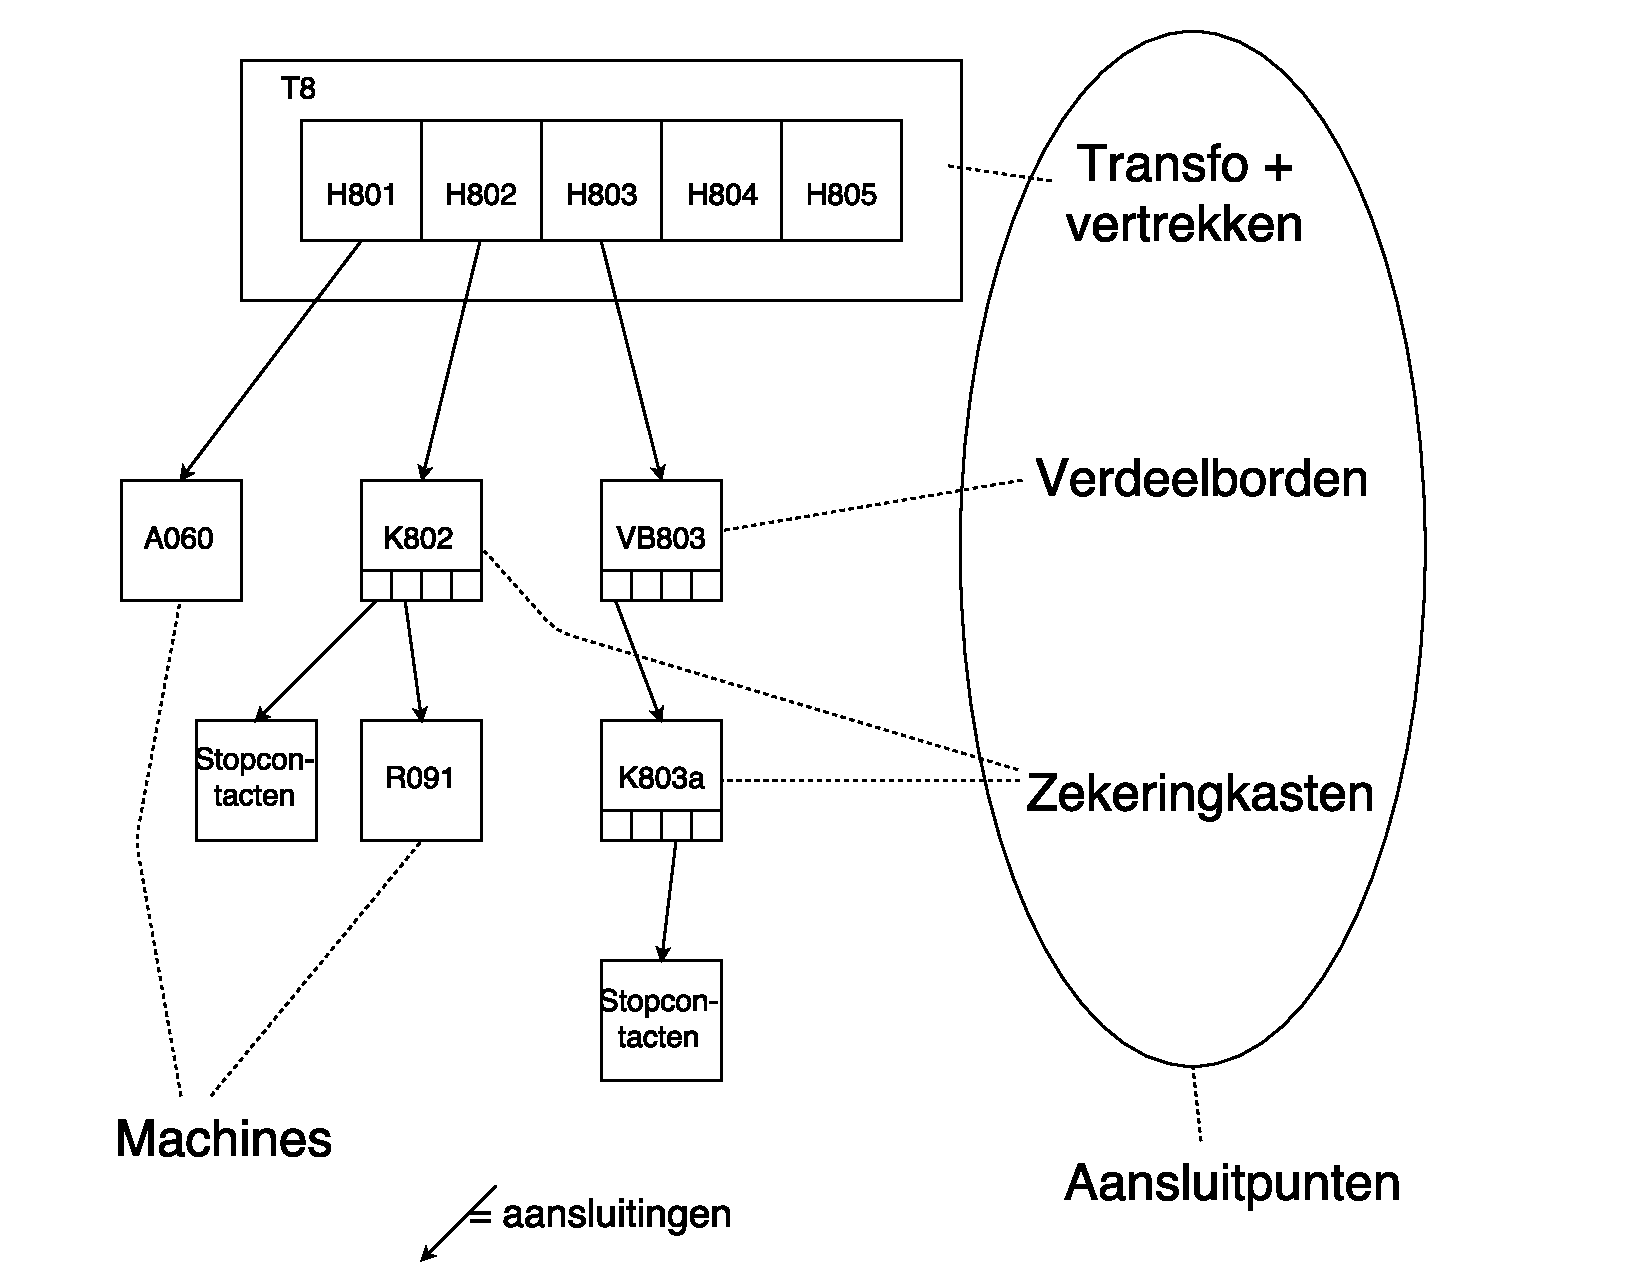
\includegraphics[width=1.2\textwidth]{pictures/Aansluitpunten.ps}
%\end{homeworkProblem}
%\newpage

\begin{homeworkProblem}[Database]
\begin{itemize}
\item\textbf{Doel} : alle communciatie met de database verloopt via deze klasse.
\item\textbf{Atributen} 
	\begin{itemize}
        \item \textcolor{blue}{\textbf{$-$string server}}
        \item \textcolor{blue}{\textbf{$-$string database}}
        \item \textcolor{blue}{\textbf{$-$string user}}
        \item \textcolor{blue}{\textbf{$-$string password}}
        \item \textcolor{blue}{\textbf{$-$string connectiestring}}
        \item \textcolor{blue}{\textbf{$-$MySqlConnection connectie}}
	\end{itemize}
\item\textbf{Methodes}
	\begin{itemize}
	\item \textcolor{blue}{\textbf{$-$Open():bool}}
		\begin{itemize}
			\item \textbf{Doel} : openen van een connectie met de database.
			\item \textbf{Parameters} : geen.
			\item \textbf{Return} : bool 
				\begin{itemize}
					\item false = mislukt 
					\item true = connectie is geopend
				\end{itemize}
		\end{itemize}
        \item \textcolor{blue}{\textbf{$-$Close():bool}}
        	\begin{itemize}
			\item \textbf{Doel} : sluiten van de connectie met de database.
			\item \textbf{Parameters} : geen.
			\item \textbf{Return} : bool 
				\begin{itemize}
					\item false = mislukt 
					\item true = connectie is gesloten
				\end{itemize}
		\end{itemize}
	\item\textcolor{blue}{\textbf{$+$getTransfos():DataSet}}
        	\begin{itemize}
			\item \textbf{Doel} : ophalen van alle transformatoren die op het bedrijf aanwezig zijn.
			\item \textbf{Parameters} : geen.
			\item \textbf{Return} : DataSet met gegevens van alle transformatoren
		\end{itemize}
	\item  \textcolor{blue}{\textbf{$+$getAansluitingen(String aansluitpunt):DataSet}}
		\begin{itemize}
                        \item \textbf{Doel} : opvragen van alle aansluitingen die behoren tot een bepaalde aansluitpunt
                        \item \textbf{Parameters} : String aansluitpunt
                        \item \textbf{Return} : DataSet met gegevens van alle aansluitingen van een aansluitpunt
                \end{itemize}
	\item  \textcolor{blue}{\textbf{$+$getSearch(String search):DataSet}}
		\begin{itemize}
                        \item \textbf{Doel} : ophalen van zoekresultaten
                        \item \textbf{Parameters} : String search, waarbij search de zoekterm is
                        \item \textbf{Return} : DataSet met alle zoekresultaten
                \end{itemize}
	\item  \textcolor{blue}{\textbf{$+$getMachineOmschrijving(String machine):String}}
		\begin{itemize}
                        \item \textbf{Doel} : opvragen van de omschrijving van een bepaalde machine
                        \item \textbf{Parameters} : String machine
                        \item \textbf{Return} : String met de omschrijving
                \end{itemize}
        \item \textcolor{blue}{\textbf{ $+$getMachineLocatie(String machine):String}}
		\begin{itemize}
                        \item \textbf{Doel} : opvragen van de locatie van een bepaalde machine
                        \item \textbf{Parameters} : String machine
                        \item \textbf{Return} : String met de locatie
                \end{itemize}
	\item \textcolor{blue}{\textbf{ $+$getAansluitpuntLocatie(String aansluitpunt):String}}
		\begin{itemize}
                        \item \textbf{Doel} : opvragen van de locatie van een bepaalde aansluitpunt
                        \item \textbf{Parameters} : String aansluitpunt
                        \item \textbf{Return} : String met de locatie
                \end{itemize}
	\item  \textcolor{blue}{\textbf{$+$getVoeding(String aansluitpunt):String}}
		\begin{itemize}
                        \item \textbf{Doel} : opvragen van de voeding van een bepaald aansluitpunt
                        \item \textbf{Parameters} : String aansluitpunt
                        \item \textbf{Return} : String met de voeding, = "-" als er geen voeding is gevonden
                \end{itemize}
	\item  \textcolor{blue}{\textbf{$+$getKabel(String aansluitpunt):String}}
		\begin{itemize}
                        \item \textbf{Doel} : opvragen van de voedingskbal van een bepaald aansluitpunt
                        \item \textbf{Parameters} : String aansluitpunt
                        \item \textbf{Return} : String met de voedingskabel, = "-" als er geen voedingskabel is gevonden
                \end{itemize}
	\item \textcolor{blue}{ \textbf{$+$getStroom(String aansluitpunt):String}}
		\begin{itemize}
                       \item \textbf{Doel} : opvragen van de stroomtoevoer (voeding) van een bepaald aansluitpunt
                        \item \textbf{Parameters} : String aansluitpunt
                        \item \textbf{Return} : String met de stroom, = "-" als er geen voeding is gevonden
                \end{itemize}
	\item  \textcolor{blue}{\textbf{$+$setAansluitingen(DataSet dsDatabase):bool}}
		\begin{itemize}
                        \item \textbf{Doel} : data van alle aansluitingen van een aansluitpunt opslaan in de database
                        \item \textbf{Parameters} : DataSet dsDatabase met alle aansluitingen van een aansluitpunt
                        \item \textbf{Return} : bool
				\begin{itemize}
                                        \item false = mislukt
                                        \item true = connectie is gesloten
                                \end{itemize}
                \end{itemize}
	\end{itemize}
\end{itemize}
\end{homeworkProblem}

\begin{homeworkProblem}[Hoofdscherm]
\begin{itemize}
\item\textbf{Doel} : Het hoofdscherm van het programma opbouwen. Dez klasse
communiceert met de \textbf{Database}-klasse om de nodige gegevens uit de
database op te halen. Andere vensters worden van uit deze klasse aangeroepen.
\item\textbf{Atributen}
        \begin{itemize}
	\item \textcolor{blue}{\textbf{$-$Database database}} : Alle communicatie met de database verloopt via de database klasse
        \item \textcolor{blue}{\textbf{$-$DataTable dtDisplay}} : Inhoud van deze DataTable wordt via een DataGridView op het scherm getoond
        \item \textcolor{blue}{\textbf{$-$bool unsaved}} : Staan er niet bewaarde gegevens op het scherm?
        \item \textcolor{blue}{\textbf{$-$string aansluitpunt}} : Het aansluitpunt dat momenteel wordt getoond
\end{itemize}
\item\textbf{Methodes}
	\begin{itemize}


        \item  \textcolor{blue}{\textbf{$-$showTransfos()}}
		\begin{itemize}
                        \item \textbf{Doel} : Tonen van overzicht van alle transfos op het scherm
                        \item \textbf{Parameters} : geen.
                        \item \textbf{Return} : niets.
		\end{itemize}

	\item  \textcolor{blue}{\textbf{$-$showAansluitpunt(String aansluitpunt)}}
		\begin{itemize}
                        \item \textbf{Doel} : Tonen van alle aansluitingen van een bepaald aansluitpunt
                        \item \textbf{Parameters} : String aansluitpunt
                        \item \textbf{Return} : niets.
                \end{itemize}

	\item  \textcolor{blue}{\textbf{$-$showSearch(String search)}}
                \begin{itemize}
                        \item \textbf{Doel} : Tonen van de zoekresultaten
                        \item \textbf{Parameters} : String met de zoekterm
                        \item \textbf{Return} : niets.
                \end{itemize}

        \item  \textcolor{cyan}{\textbf{$-$showCommon(String word, int
modus)}} 
		\begin{itemize}
                        \item \textbf{Doel} : Tijdens het programmeren is
gebleken dat er veel code gemeenschappelijk is tussen \textbf{showTransfos},
\textbf{showAansluitpunt}, \textbf{showSearch}, daarom is deze
gemeenschappelijke routine aangemaakt.
                        \item \textbf{Parameters} : String
zoekterm/aansluitpunt, int modus 1=Transfos, 2=Aansluitpunt, 3=Search
                        \item \textbf{Return} : niets.
                \end{itemize}

	
	\item \textcolor{blue}{\textbf{$-$dgvLaagspanningsnet\_CellContentClick(object sender, DataGridViewCellEventArgs e)}}
                \begin{itemize}
                        \item \textbf{Doel} : Actie ondernemen als er op een Cell van de DataGridView wordt geklikt
                        \item \textbf{Parameters} : object sender, DataGridViewCellEventArgs e
                        \item \textbf{Return} : niets.
                \end{itemize}

	\item  \textcolor{blue}{\textbf{$-$btnDynVoeding\_Click(object sender, EventArgs e)}}
                \begin{itemize}
                        \item \textbf{Doel} : Actie ondernemen als er op de voedingsknop is geklikt
                        \item \textbf{Parameters} : object sender, EventArgs e
                        \item \textbf{Return} : niets.
                \end{itemize}

	\item  \textcolor{blue}{\textbf{$-$setUnsaved(bool status)}}
                \begin{itemize}
                        \item \textbf{Doel} : Bijhouden of data reeds in de database is opgeslagen
                        \item \textbf{Parameters} : bool status
				\begin{itemize}
					\item false : database- en scherm-inhoud komen overeen
					\item true : niet alle gegevens zijn bewaard
				\end{itemize}
                        \item \textbf{Return} : niets.
                \end{itemize}
	\item  \textcolor{cyan}{\textbf{$-$dgvLaagspanningsnet\_SelectionChanged(object sender, EventArgs e)}}
                \begin{itemize}
                        \item \textbf{Doel} : Uitschakelen van blauwe
selectiebalk in DataGridView\\ (zie ook: https://stackoverflow.com/questions/11330147/how-to-disable-the-ability-to-select-in-a-datagridview)
                        \item \textbf{Parameters} : object sender, EventArgs e
                        \item \textbf{Return} : niets.
                \end{itemize}

	\item  \textcolor{blue}{\textbf{$-$btnSave\_Click(object sender, EventArgs e)}}
		\begin{itemize}
			\item \textbf{Doel} : Actie ondernemen als er op de save-knop wordt geklikt
			\item \textbf{Parameters} : object sender, EventArgs e
			\item \textbf{Return} : niets.
		\end{itemize}

       \item  \textcolor{blue}{\textbf{$-$btnUndo\_Click(object sender, EventArgs e)}}
                \begin{itemize}
                        \item \textbf{Doel} : Actie ondernemen als er op de undo-knop wordt geklikt
                        \item \textbf{Parameters} : object sender, EventArgs e
                        \item \textbf{Return} : niets.
                \end{itemize}

	\item  \textcolor{blue}{\textbf{$-$btnSearch\_Click(object sender, EventArgs e)}}
                \begin{itemize}
                        \item \textbf{Doel} : Actie ondernemen als er op de zoek-knop wordt geklikt
                        \item \textbf{Parameters} : object sender, EventArgs
                        \item \textbf{Return} : niets.
                \end{itemize}

	\item \textcolor{cyan}{\textbf{$-$txtbxSearch\_KeyDown(object sender, KeyEventArgs e)}}
		\begin{itemize}
                        \item \textbf{Doel} : Op Enter drukken in de search box = op zoekknop klikken.
                        \item \textbf{Parameters} : object sender, EventArgs
                        \item \textbf{Return} : niets.
                \end{itemize}
	\end{itemize}
\end{itemize}
\end{homeworkProblem}

\end{document}
